\documentclass[10pt]{beamer}
\usepackage{amsmath}
\usepackage{mathtools}
%\documentclass[12pt]{beamerthemeSam.sty}
\usepackage{epsf}
%\usepackage{pstricks}
%\usepackage[orientation=portrait,size=A4]{beamerposter}
\geometry{paperwidth=160mm,paperheight=120mm}
%DT favorite definitions
\def\LL{\left\langle}	% left angle bracket
\def\RR{\right\rangle}	% right angle bracket
\def\LP{\left(}		% left parenthesis
\def\RP{\right)}	% right parenthesis
\def\LB{\left\{}	% left curly bracket
\def\RB{\right\}}	% right curly bracket
\def\PAR#1#2{ {{\partial #1}\over{\partial #2}} }
\def\PARTWO#1#2{ {{\partial^2 #1}\over{\partial #2}^2} }
\def\PARTWOMIX#1#2#3{ {{\partial^2 #1}\over{\partial #2 \partial #3}} }

\def\rightpartial{{\overrightarrow\partial}}
\def\leftpartial{{\overleftarrow\partial}}
\def\diffpartial{\buildrel\leftrightarrow\over\partial}

\def\BI{\begin{itemize}}
\def\EI{\end{itemize}}
\def\BE{\begin{displaymath}}
\def\EE{\end{displaymath}}
\def\BEA{\begin{eqnarray*}}
\def\EEA{\end{eqnarray*}}
\def\BNEA{\begin{eqnarray}}
\def\ENEA{\end{eqnarray}}
\def\EL{\nonumber\\}


\newcommand{\map}[1]{\frame{\frametitle{\textbf{Course map}}
\centerline{\includegraphics[height=0.86\paperheight]{../../map/#1.png}}}}
\newcommand{\wmap}[1]{\frame{\frametitle{\textbf{Course map}}
\centerline{\includegraphics[width=0.96\paperwidth]{../../map/#1.png}}}}

\newcommand{\etal}{{\it et al.}}
\newcommand{\gbeta}{6/g^2}
\newcommand{\la}[1]{\label{#1}}
\newcommand{\ie}{{\em i.e.\ }}
\newcommand{\eg}{{\em e.\,g.\ }}
\newcommand{\cf}{cf.\ }
\newcommand{\etc}{etc.\ }
\newcommand{\atantwo}{{\rm atan2}}
\newcommand{\Tr}{{\rm Tr}}
\newcommand{\dt}{\Delta t}
\newcommand{\op}{{\cal O}}
\newcommand{\msbar}{{\overline{\rm MS}}}
\def\chpt{\raise0.4ex\hbox{$\chi$}PT}
\def\schpt{S\raise0.4ex\hbox{$\chi$}PT}
\def\MeV{{\rm Me\!V}}
\def\GeV{{\rm Ge\!V}}

%AB: my color definitions
%\definecolor{mygarnet}{rgb}{0.445,0.184,0.215}
%\definecolor{mygold}{rgb}{0.848,0.848,0.098}
%\definecolor{myg2g}{rgb}{0.647,0.316,0.157}
\definecolor{abtitlecolor}{rgb}{0.0,0.255,0.494}
\definecolor{absecondarycolor}{rgb}{0.0,0.416,0.804}
\definecolor{abprimarycolor}{rgb}{1.0,0.686,0.0}
\definecolor{Red}           {cmyk}{0,1,1,0}
\definecolor{Grey}           {cmyk}{.7,.7,.7,0}
\definecolor{Blue}          {cmyk}{1,1,0,0}
\definecolor{Green}         {cmyk}{1,0,1,0}
\definecolor{Brown}         {cmyk}{0,0.81,1,0.60}
\definecolor{Black}         {cmyk}{0,0,0,1}

\usetheme{Madrid}


%AB: redefinition of beamer colors
%\setbeamercolor{palette tertiary}{fg=white,bg=mygarnet}
%\setbeamercolor{palette secondary}{fg=white,bg=myg2g}
%\setbeamercolor{palette primary}{fg=black,bg=mygold}
\setbeamercolor{title}{fg=abtitlecolor}
\setbeamercolor{frametitle}{fg=abtitlecolor}
\setbeamercolor{palette tertiary}{fg=white,bg=abtitlecolor}
\setbeamercolor{palette secondary}{fg=white,bg=absecondarycolor}
\setbeamercolor{palette primary}{fg=black,bg=abprimarycolor}
\setbeamercolor{structure}{fg=abtitlecolor}

\setbeamerfont{section in toc}{series=\bfseries}

%AB: remove navigation icons
\beamertemplatenavigationsymbolsempty
\title[Energy: the work-energy theorem]{
  \textbf {Energy: the work-energy theorem}\\
%\centerline{}
%\centering
%\vspace{-0.0in}
%\includegraphics[width=0.3\textwidth]{propvalues_0093.pdf}
%\vspace{-0.3in}\\
%\label{intrograph}
}

\author[W. Freeman] {Physics 211\\Syracuse University, Physics 211 Spring 2015\\Walter Freeman}

\date{\today}

\begin{document}

\frame{\titlepage}

\frame{\frametitle{\textbf{Announcements}}
\BI
\large
\item{Exams will be returned tomorrow in recitation}
\item{Exam stats etc. will be posted once I have them all}
  \BI
   \item{I think a lot of people forgot things about forces over spring break}
\item{Also, I hear there are some basketball teams wrecking faces and taking names...}
\item{If you didn't do so well, there's always the makeup}
  \EI
\item{Next homework will be posted today or Friday and due next Friday.}
\EI
}

\frame{\frametitle{\textbf{Makeup exam}}
\BI
\large
\item{Our usual makeup exam will be held in two weeks}
\item{However, lots of people were sick on Tuesday -- there is something nasty going around}
\item{Anyone who did not take the exam due to documented illness can take a special makeup}
\item{If that's you, email me your availability:}
\BI
\item{Saturday morning}
\item{Saturday afternoon}
\item{Sunday afternoon}
\item{Monday morning}
\item{Monday afternoon}
\item{Monday night}
\EI
\EI
}

\frame{\frametitle{\textbf{Energy methods, in general}}
\large
\BI
\item{``Conventional'' kinematics: compute $\vec x(t)$, $\vec v(t)$}
  \BI
\item{``Time-aware'' and ``path-aware'' -- tells us the history of a thing's movement}
\item{Time is an essential variable here}
  \EI
\item{Newton's second law: forces $\rightarrow$ acceleration $\rightarrow$ history of movement}
\item{Sometimes we don't care about all of this}
\item{Roll a ball down a track: how fast is it going at the end?}
\EI
}

\frame{\frametitle{\textbf{Energy methods, in general}}
\large
We will see that things are often simpler when we look at something called ``energy''
\BI
\item{Basic idea: don't treat $\vec a$ and $\vec v$ as the most interesting things any more}
\item{Treat $v^2$ as fundamental: $\frac{1}{2}mv^2$ called ``kinetic energy''}
  \EI
  \bigskip
  \begin{columns}
    \column{0.5\textwidth}
    \color{Blue}
    \centerline{Previous methods:}
    \BI
    \color{Blue}
  \item{Velocity is fundamental}
  \item{Force: causes velocities to change over time}
  \item{Intimately concerned with vector quantities}
  \EI
    \column{0.5\textwidth}
    \color{Red}
    \centerline{Energy methods:}
    \BI
    \color{Red}
  \item{$v^2$ (related to kinetic energy) is fundamental}
  \item{Force: causes KE to change over distance}
  \item{Energy is a {\it scalar}}
    \EI
  \end{columns}
  
  \bigskip
  \bigskip
  
  \centerline{Energy methods: useful when you don't know and don't care about time}
}

\frame{\frametitle{\textbf{The work-energy theorem in 1D}}

  \Large
  We've encountered something before that eliminates time as a variable...

\pause

\bigskip

The ``third kinematics relation''
\begin{equation*}
  v_f^2 - v_0^2 = 2a\Delta x
\end{equation*}

\pause
\bigskip

Multiply by $\frac{1}{2}m$:

\begin{equation*}
  \frac{1}{2} mv_f^2 - \frac{1}{2} mv_0^2 = am\, \Delta x
\end{equation*}

That thing on the right looks familiar...

}

\frame{\frametitle{\textbf{The work-energy theorem in 1D}}
  \Large
We've encountered something before that eliminates time as a variable...

\pause

\bigskip

The ``third kinematics relation''

\begin{equation*}
  v_f^2 - v_0^2 = 2a\Delta x
\end{equation*}

\pause
\bigskip

Multiply by $\frac{1}{2}m$:

\begin{equation*}
  \frac{1}{2} mv_f^2 - \frac{1}{2} mv_0^2 = F \Delta x
\end{equation*}

\pause

Some new terminology:
\BI
\item{$\frac{1}{2}mv^2$ called the ``kinetic energy'' (positive only!)}
\item{$F \Delta x$ called the ``work'' (negative or positive!)}
\item{``Work is the change in kinetic energy''}
\EI
}

\frame{\frametitle{\textbf{Sample problem: dropping an object}}
\Large
\centerline{A rather clumsy cat falls off of a cat tree 2m high.}
\centerline{At what speed does he hit the ground?}
\normalsize

\bigskip
\pause

\centerline{Feet first, of course -- we're not cruel!}

\bigskip
\bigskip
\bigskip
\bigskip
\Large

\centerline{$KE_f - KE_0 = F \Delta y$}
\pause

\BI
\item{$KE_0 = 0$}
\item{Work done by gravity: $(-h) \times (-mg) = mgh$}
\item{$KE_f - KE_0 = mgh \rightarrow v_f = \sqrt{2gh} = 6.26 \rm m/\rm s$}
  \EI
}

\frame{\frametitle{\textbf{Sample problem: Baseball problem (exam 1)}}
\Large
\centerline{I throw a ball straight up with initial speed $v_0$.}
\centerline{Someone catches it at height $h$. How fast is it going?}
\pause

\bigskip
\bigskip
\bigskip
\bigskip

\BI
\item{$\frac{1}{2}mv_f^2 - \frac{1}{2}mv_0^2 = (-mg) \times h$}
\item{... algebra follows: solve for $v_f$}
\EI
}

\frame{\frametitle{\textbf{Multiple pendulum demo}}
  \Large
  \centerline{The total work done is zero!}
\bigskip
\bigskip
\bigskip
\centerline{One side has a large $\Delta s$ and a small $F$.}
\centerline{One side has a small $\Delta s$ and a large $F$.}
}



\frame{\frametitle{\textbf{Work-energy theorem: 2D}}
  \large
  \centerline{We can do this in two dimensions, too:}
  \BI
\item{$\frac{1}{2}mv_{x,f}^2 - \frac{1}{2}mv_{x,0}^2 = F_x \Delta x$}
\item{$\frac{1}{2}mv_{y,f}^2 - \frac{1}{2}mv_{y,0}^2 = F_y \Delta y$}
  \EI

\bigskip
\bigskip
\bigskip

\centerline{Add these together:}
\BI
\item{$\frac{1}{2}m(v_{x,f}^2 + v_{y,f}^2) - \frac{1}{2}m(v_{x,0}^2 + v_{y,0}^2) = F_x \Delta x + F_y \Delta y$}
  \pause

\bigskip
\bigskip
\bigskip

\item{The thing on the left can be simplified with the Pythagorean theorem:}
\item{$\frac{1}{2}m(v_f^2) - \frac{1}{2}mv_0^2 = F_x \Delta x + F_y \Delta y$}

\bigskip
\bigskip

\item{That funny thing on the right is called a ``dot product''.}
  \EI
}

\frame{\frametitle{\textbf{Dot products}}
  \large
  \centerline{  $A_x B_x + A_y B_y$ is written as $\vec A \cdot \vec B$.}

\bigskip
\bigskip

\normalsize
What does this mean? It's a way of ``multiplying'' two vectors to get a scalar (a number).

\pause

We can choose coordinate axes as always: choose them to align either with $\vec F$ or $\Delta \vec s$.

\bigskip

\begin{columns}
\normalsize
  \column{0.5\textwidth}
  \centerline{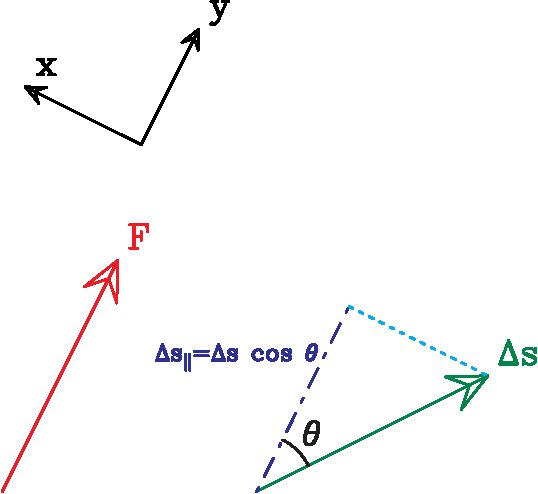
\includegraphics[width=0.6\textwidth]{dp1-crop.pdf}}
  \BI
\item{$\vec F \cdot \Delta \vec s = (F) (\Delta s_\parallel) = (F) (\Delta s \cos \theta)$}
\item{``The component of the displacement parallel to the force, times the force}
  \EI

  \column{0.5\textwidth}
  \centerline{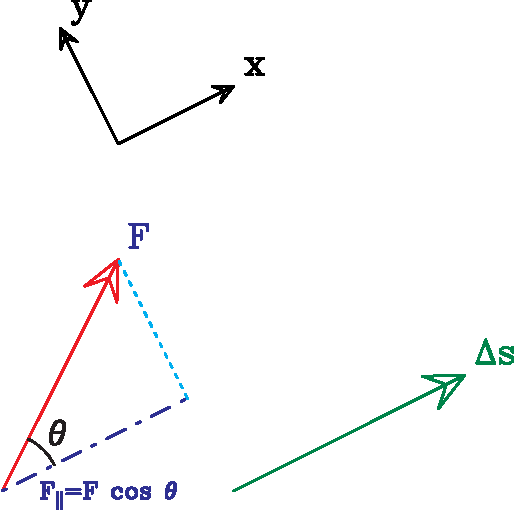
\includegraphics[width=0.6\textwidth]{dp2-crop.pdf}}
  \BI
\item{$\vec F \cdot \Delta \vec s = (F_\parallel) (\Delta s) = (F \cos \theta) (\Delta s)$}
\item{``The component of the force parallel to the motion, times the displacement}
  \EI


\end{columns}
\large
\bigskip
\centerline{\color{Red}Different cases where each form is useful, but it's the same trig either way}
}
\frame{\frametitle{\textbf{Pendulum demos}}
  \large
  \BI
\item{What is the work done by the string?}
  \pause
\item{\color{Red}Zero -- it's always perpendicular to the motion!}
\item{How high will it swing on the other side?}
  \pause
\item{Gravity does positive work on the way down and negative work on the way up}
\item{The kinetic energy can't go below zero}
\item{The height at each end of the swing must be the same!}
\item{... and the return height can't be greater than the initial height...}
\EI
\pause
\bigskip
\bigskip

\normalsize
\centerline{\color{Blue}(If physics stops working and I go splat, have a nice summer!}
}


\frame{\frametitle{\textbf{Ball rolling down a ramp demo}}
    \BI
    \large
  \item{What is the work done by the normal force?}
    \pause
  \item{\color{Red}Zero -- the normal force is always perpendicular to the motion!}
  \item{What is the work done by gravity?}
    \pause
  \item{Use the ``force times parallel component of motion'' formulation:}
    
  \item{$W = (-mg) \times (y_f - y_0)$ -- note both components are negative, for a positive result}
  \item{The shape of the ramp doesn't matter: the velocities will all be the same at the end!}
    \EI
}

\frame{\frametitle{\textbf{Another sample problem}}
\Large
A car slams on its brakes going a speed $v_0$. How far does it travel before it stops?
}


\frame{\frametitle{\textbf{Hot Wheels demo}}
  \large
  \centerline{How does the velocity at the middle photogate relate to that at the bottom?}
  \pause

\bigskip
\bigskip
\bigskip

\centerline{All I need are the heights; the shape doesn't matter at all!}

\bigskip
\bigskip
\bigskip

\pause

Middle: Work done by gravity = $mg(1h)$, $\frac{1}{2}mv^2 = mg(1h), v = \sqrt{2gh}$\\
Bottom: Work done by gravity = $mg(2h)$, $\frac{1}{2}mv^2 = mg(2h), v = \sqrt{4gh}$\\

\bigskip

\centerline{The velocity at the bottom is larger by a factor of $\sqrt{2}$!}
}

\end{document} 
